\section{DESENVOLVIMENTO EXPERIMENTAL}
\subsection{Materiais e Metodos}
Para a realização do experimento, foram utilizados
\begin{itemize}
	\item Mini-laser;
	\item Mesa de alinhamento;
	\item Uma lente de 48 mm;
	\item Uma lente de 252 mm;
	\item Um separador de feixe;
	\item Um espelho de alta rotação PASCO OS-9263B;
	\item Um espelho fixo esferico com raio de 13.5 m;
\end{itemize}
Sendo o experimento montado da seguinte forma:
\begin{figure}[h!]
	\centering
	\fbox{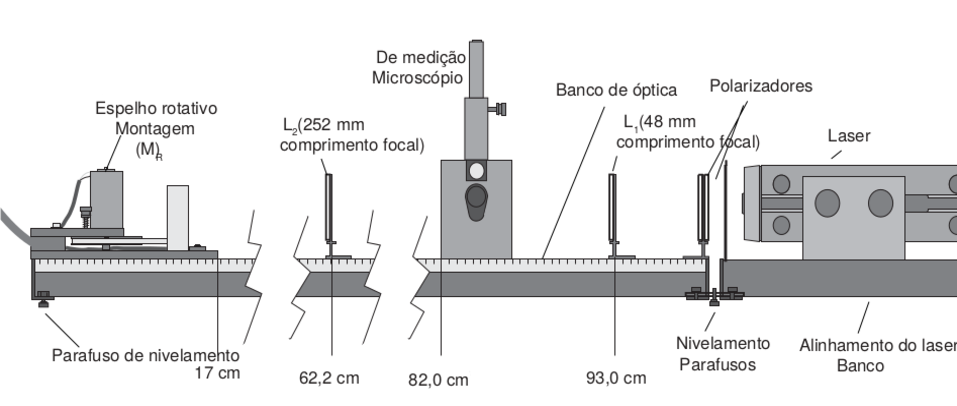
\includegraphics[scale= 0.35]{mtg}}
	\caption{Montagem Experimental utilizada}
\end{figure}


Primeiro é posto o laser e o espelho rotativo, então são alinhados
utilizando gabaritos, após esta etapa, é posta a primeira lente,
alinhado novamente o plano do laser, posto o separador de feixe, e
então a segunda lente e feito novamente as correções de alinhamento,
para colocar todos os objetos opticos em um mesmo plano. Seguindo,
utilizando regras trigonométricas, é posto o espelho esferico 9 metros
do espelho rotatorio aproximadamente, e formando um angulo de 12º
entre os feixes, e após ser posto, o espelho rotatorio é direcionado
no centro do espelho fixo, é verificado o alinhamento do sistema, e se
está tendo retorno no separador de feixes, para isto, é removido o
microscopio do separador, posto um papel de pequena gramatura no
local, e então bloqueado o feixe de luz após o espelho rotario, e um
ponto sumindo no papel, significa o exito no alinhamento. Por fim, é
recolocado o miscroscopio e então alinhado utilizando o micrometro com
o centroda visão.
\subsection{Dados experimentais}
Após a reaização do experimento foram obtidos os seguintes dados
\begin{table}[h!]
\centering

\begin{tabular}{|	c	|	c	|}
\hline
$\Delta$ s' & $f$   \\ \hline
14          & 750   \\ \hline
30          & 1500  \\ \hline
-15         & -750  \\ \hline
-30         & -1500 \\ \hline
\end{tabular}
\caption{Dados obtidos}
\end{table}
Utilizando os dados obtidos, foi construido um gráfico e fazendo o
ajuste linear é possivel obter a equação da reta $\Delta s
=0.02\times10^{-8}f$.

Sabendo que
\begin{equation}
	c = \frac{4AD^22\pi f}{(D+B)\Delta s}
\end{equation}
é possivel fazer
\begin{equation}
\begin{split}
	\Delta s = \frac{4AD^22\pi f}{(D+B)c}\\
	\Delta s = 2\times10^{-10}f
\end{split}
\end{equation}
portante
\begin{equation}
\begin{split}
	2\times10^{-10}=\frac{8AD^2\pi}{(D+B)c}\\
	c=\frac{8AD^2\pi}{(D+B)2\times10^{-10}}
\end{split}
\end{equation}
substituindo os valores obtidos
\begin{equation}
	\begin{split}
		A = 0,261 m \pm 0,0
	\end{split}
\end{equation}
\subsection{Interpretação dos resultados}

aaaaaaaaaaaaaaaaaaaaaaa
